\section{Ejercicio 2: filtrado por convolución}
Se desea implementar el filtro desarrollado en la sección anterior mediante convolución. Este algoritmo tiene base en realizar una FFT de la entrada y respuesta impulsiva, para luego realizar el producto de las mismas en el marco espectral y anti-transformar (IFFT) el resultado, obteniendo así la salida del filtro:


\vspace{0.5cm}
\begin{figure}[H]
  \centering
  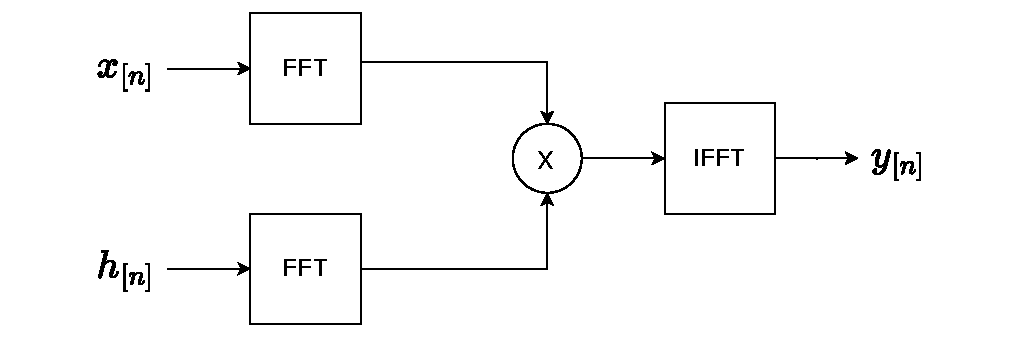
\includegraphics[width = 0.7 \textwidth]{Imagenes/2_conv/esquema_basico.pdf}
  \caption{Esquema básico de filtrado por convolución}
  \label{fig:  Esquema básico de filtrado por convolución}
\end{figure}

\noindent En función de que el algoritmo de FFT es O(n . log(n)) se busca optimizar el cálculo. 

Si bien la operatoria parecería estar completamente definida bajo este esquema, si se requiere procesar la entrada en bloques se han de tener ciertas consideraciones. Para llegar a ellas debemos partir de la cuenta que se ha de realizar en el marco temporal. Si el filtro dispone de M coeficientes:

\begin{align*}
    y[n] = \sum_{k=0}^{M-1}h[k] \cdot x[n-k]
\end{align*}

\noindent lo cual corresponde con la operatoria habitual. Sin embargo, a la hora de emplear la DFT (o, en su defecto, la FFT) se realiza una extensión periódica de la señal, por lo que la operación desplazamiento no se condice con le expresión previamente indicada. A la operación que se debe realizar se la conoce como \emph{convolución circular}, mientras que la que se realiza habitualmente lleva el nombre de \emph{convolución lineal}. Esto parecería no tener relevancia para con la cuenta que se ha de efectuar en esta técnica, pues le compete al marco temporal y no al espectral (donde en principio tiene pie este proceso); sin embargo, esto es relevante para determinar la longitud de la FFT a realizar. 

De querer filtrar una señal $x[n]$ de longitud L mediante el filtro previamente descrito ($h[n]$ de longitud M), la salida asociada tendría una longitud $L+M-1$. De este modo, si se toma una cantidad de muestras $N$ para realizar la FFT tal que sea menor que $L+M-1$ el cálculo seria erróneo. Para visualizarlo tomemos un ejemplo sencillo:

\begin{align*}
    &x[n] = {1,1} \\
    &h[n] = {1,1}
\end{align*}

\noindent aquí L=M=2. Si realizamos la convolución lineal y calculamos $y[0]$, observamos que:

\begin{align*}
    y[0] = x[0] \cdot h[0] + x[1] \cdot h[-1] = 1 \cdot 1 + 1 \cdot 0 = 1
\end{align*}

\noindent si ahora tomamos $N=2$, la relación que se mantiene es la misma, pero la señal temporal asociada a la señal espectral obtenida con la DFT no tiene $h[-1]=0$, sino que $h[1] = 1$. De este modo:

\begin{align*}
    y[0] = x[0] \cdot h[0] + x[1] \cdot h[-1] = 1 \cdot 1 + 1 \cdot 1 = 2 \neq 1
\end{align*}

\noindent de este modo, resulta evidente el problema que se estaba desarrollando. En vista a esto, la conclusión es que se ha de realizar un padding con ceros a la hora de calcular la FFT con tal de que la cuenta en el marco espectral se condiga con la cuenta deseada en el marco temporal. Consecuentemente se realiza una FFT de al menos $L+M-1$ muestras. Siendo que la FFT es un algoritmo de cálculo de la DFT que resulta eficiente en con tamaños potencias de dos, es posible ajustar $N$ tal que se den ambas condiciones simultáneamente. En este caso particular, siendo $L =1024$ y $M=527$, se puede tomar $N=2048$.

Hasta aquí se concluyo la necesidad de añadir ceros adicionales para poder efectuar la cuenta correspondiente sin error. No obstante resta analizar dónde se han de colocar estos ceros, al igual que como se han de procesar los subsecuentes bloques. Existen dos técnicas que definen estos comportamientos: 

\begin{itemize}
    \item Overlap and save.
    \item Overlap and add.
\end{itemize}

En este informe se desarrollará el primero de ellos. 

\subsection{Overlap and save}

Por un lado, la respuesta impulsiva a transformar dispone de N-M ceros adicionales en su cola:

\vspace{0.5cm}
\begin{figure}[H]
  \centering
  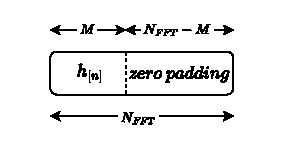
\includegraphics[width = 0.5 \textwidth]{Imagenes/2_conv/h_overlap_and_save.drawio.pdf}
  \caption{Respuesta impulsiva a transformar.}
  \label{fig: rta impulsiva a transformar}
\end{figure}

\noindent notar que la transformación de este bloque se efectúa una única vez (si se dispone de HW dedicado se puede almacenar únicamente esta transformada en lugar de los coeficientes de la respuesta impulsiva). 

En tanto a la señal de entrada, se han de tomar también N muestras, siendo relevante estudiar cuales de ellas. En la primera iteración se colocan $M-1$ ceros al comienzo del bloque, de lo contrario la cuenta efectiva con la FFT emplearía los elementos de la cola del bloque (recordar la extensión periódica que realiza esta operación). Luego de este padding se dispone de las primeras L muestras a procesar y se completa el bloque con ceros hasta alcanzar N muestras. En las siguientes iteraciones, al igual que cuando se realiza la convolución lineal, se han de tomar las M-1 muestras del bloque previo, junto con las siguientes L muestras a procesar + zero padding:

\vspace{0.5cm}
\begin{figure}[H]
  \centering
  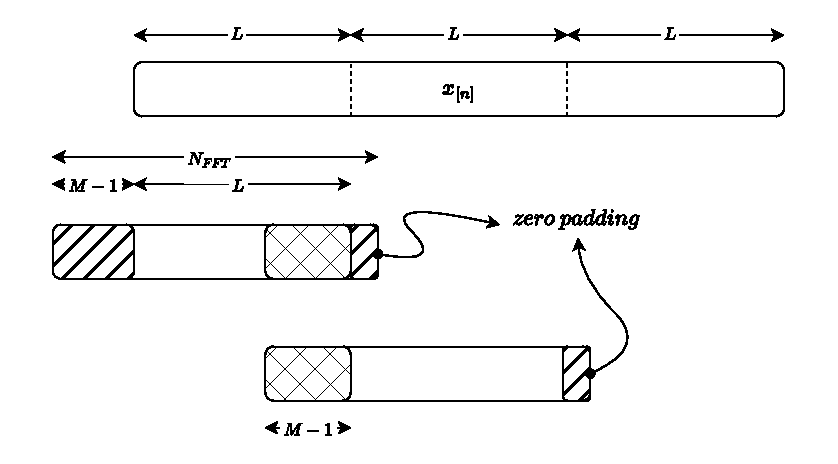
\includegraphics[width = 0.8\textwidth]{Imagenes/2_conv/bloques_entrada.pdf}
  \caption{Armado de bloques de entrada.}
  \label{fig: armado de bloques de entrada}
\end{figure}

\noindent Finalmente para con la salida, en cada iteración se obtiene $N$ muestras a partir de la IFFT, de estas $N$ muestras las primeras $M-1$ no son válidas (por la misma razón que se comentó anteriormente), al igual que las últimas $N-(L-M-1)$:

\vspace{0.5cm}
\begin{figure}[H]
  \centering
  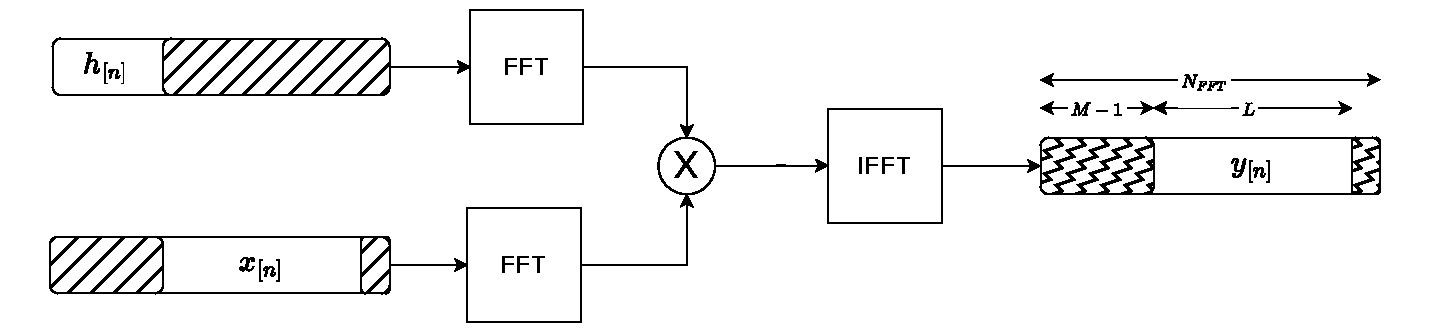
\includegraphics[width = \textwidth]{Imagenes/2_conv/diagrama_de_flujo.pdf}
  \caption{Diagrama de flujo.}
  \label{fig: diagrama de flujo}
\end{figure}


\subsection{Implementación}
Con tal de implementar el método desarrollado se hizo uso del siguiente código:

\vspace{0.5cm}
\begin{lstlisting}[style=mystyle, caption={Código empleado en la implementación.}, label={lst:filtro + ds}]
import numpy as np
import time

# --- Datos de entrada (asumiendo que ya existen) ---
# h: tus 527 coeficientes
# x: tu senal de entrada
# y_ref: el resultado de ejercicio 1 (convolucion lineal) para comparar

L = 1024
M = len(h)
N = 2048  # Potencia de 2 recomendada para h=527 y L=1024

# 1. Pre-calculo: FFT del filtro (solo una vez)
H = np.fft.fft(h, n=N)

# Inicializacion
salida_final = []
tiempos_bloque = []
pasado = np.zeros(M - 1) # M-1 ceros iniciales

# 2. Procesamiento por bloques
for i in range(0, len(x), L):
    start_time = time.perf_counter()
    
    # Tomamos el bloque actual de la senal
    bloque_actual = x[i : i + L]
    
    # Si el ultimo bloque es mas chico que L, lo rellenamos con ceros
    if len(bloque_actual) < L:
        bloque_actual = np.pad(bloque_actual, (0, L - len(bloque_actual)))
    
    # Armado del bloque de entrada N=2048: [pasado(526) + actual(1024) + ceros(498)]
    # Usamos np.concatenate o simplemente pasamos el tamano a np.fft.fft
    entrada_fft = np.concatenate([pasado, bloque_actual])
    
    # Procesamiento espectral
    X = np.fft.fft(entrada_fft, n=N)
    Y = X * H
    y_bloque = np.fft.ifft(Y).real # Nos quedamos con la parte real
    
    # --- OVERLAP AND SAVE: Salvar desde el indice M-1 hasta (M-1 + L) ---
    # Esto extrae exactamente las 1024 muestras limpias
    bloque_limpio = y_bloque[M-1 : M-1+L]
    salida_final.extend(bloque_limpio)
    
    # Actualizamos el pasado para la siguiente iteracion
    pasado = bloque_actual[-(M-1):]
    
    end_time = time.perf_counter()
    tiempos_bloque.append(end_time - start_time)

# 3. Mediciones y Comparacion
salida_final = np.array(salida_final[:len(x)]) # Recortamos al largo original si es necesario
tiempo_total = sum(tiempos_bloque)
tiempo_por_muestra = tiempo_total / len(x)

print(f"Tiempo total: {tiempo_total:.4f} s")
print(f"Tiempo por muestra: {tiempo_por_muestra:.8f} s")

# Comparacion con el ejercicio 1 (y_ref)
# Nota: y_ref debe ser recortado o comparado hasta len(x)
error = np.linalg.norm(salida_final - y_ref[:len(x)])
print(f"Error acumulado contra convolucion: {error}")
\end{lstlisting}

\noindent de este modo, se obtuvo un tiempo total de 38ms, equivalente a $0.38\mu s/muestra$ (con un error acumulado de $2\times 10^{-13}$ que se condice con un error computacional).Esta es una gran mejoria con respecto a los tiempos obtenidos en el ejercicio 1 (18.48s de procesamiento netos + $184.8\mu s$). Esta gran diferencia se debe a, por un lado, la diferencia en la complejidad computacional (O($n^2$) vs O(n log(n))), junto con un mejor empleo de los recursos (probablemente las funciones empleadas para el cálculo de la FFT e IFFT esten optimizadas, no así el código implementado en el ejercicio 1 con los dos for anidados).